\documentclass[12pt]{article}
\usepackage{graphicx}
\usepackage{listings}
\begin{document}

\begin{titlepage}

\newcommand{\HRule}{\rule{\linewidth}{0.5mm}}

\center 
\textsc{\LARGE Universitatea Tehnica din Moldova}\\[1.5cm] \textsc{\Large Raport}\\[0.5cm] 
\textsc{\large la lucrarea de laborator nr. 2 \\la disciplina "MIDPS"}\\[0.5cm]
\HRule \\[0.4cm]
{ \huge \bfseries Version Control Systems si modul de setare a unui server}\\[0.4cm]
\HRule \\[1.5cm]
\begin{minipage}{0.4\textwidth}
\begin{flushleft} \large
\emph{A efectuat:}\\
stud. gr. TI-145\\
Ialticenco \textsc{Alexandr}
\end{flushleft}
\end{minipage}
~
\begin{minipage}{0.4\textwidth}
\begin{flushright} \large
\emph{A verificat:} \\
lector univ.\\
Cojocaru \textsc{Svetlana}
\end{flushright}
\end{minipage}\\[4cm]
\vfill 
{\large Chisinau, 2016}\\[10cm] 
\end{titlepage}
\section*{Obiectivele lucrarii}
\begin{itemize}
\item Administrarea remote a masinilor linux machine folosind SSH (remote code editing)
\item Intelegerea si folosirea CLI (basic level)
\item Version Control Systems (git / mercurial / svn)
\item Compileaza codul C/C++/Java/Python prin intermediul CLI, folosind compilatoarele gcc/g++/javac/python
\end{itemize}

\section* {Sarcina lucrarii}
\textbf{Advanced level:}
\begin{itemize}
\item seteaza un branch to track a remote origin pe care vei putea sa faci push (ex. Github, Bitbucket or custom server)
\item reseteaza un branch la commit-ul anterior
\item 	merge 2 branches
\item 	conflict solving between 2 branches
\end{itemize}

\section *{Bonus Point}
\begin{itemize}
\item Scrie un script care va compila HelloWolrdPrograms projects.	
\end{itemize}
\section {Indeplinirea task-urilor}
\subsection{Configurarea autentificarii ssh}
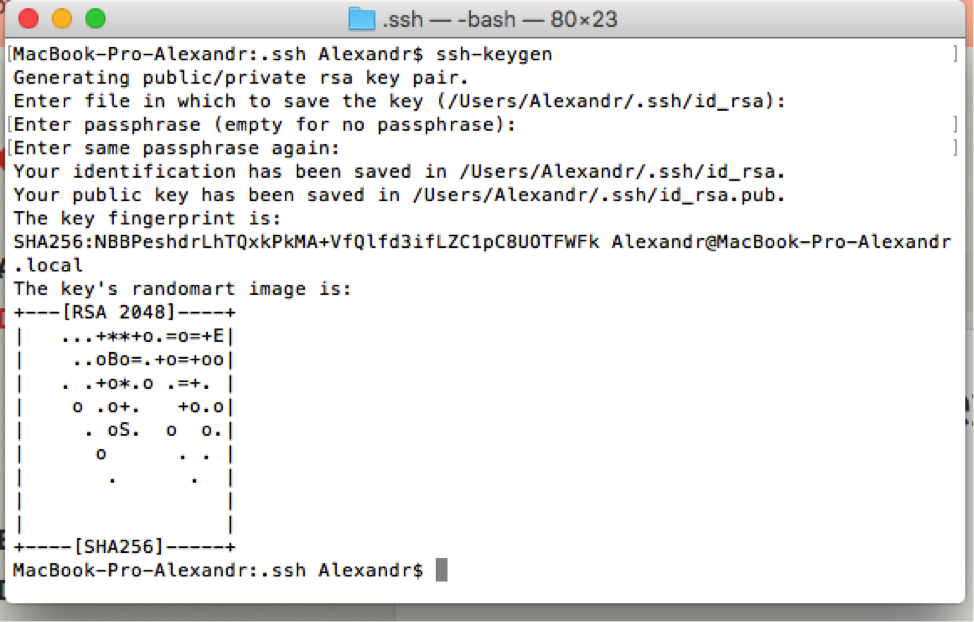
\includegraphics[width=12.5cm]{images/1}\\
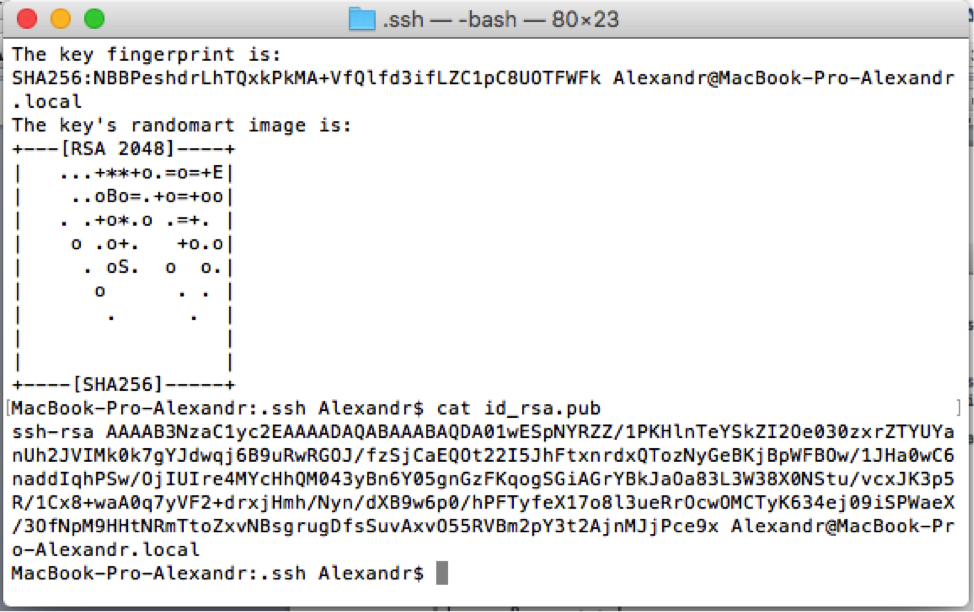
\includegraphics[width=12.5cm]{images/2}\\
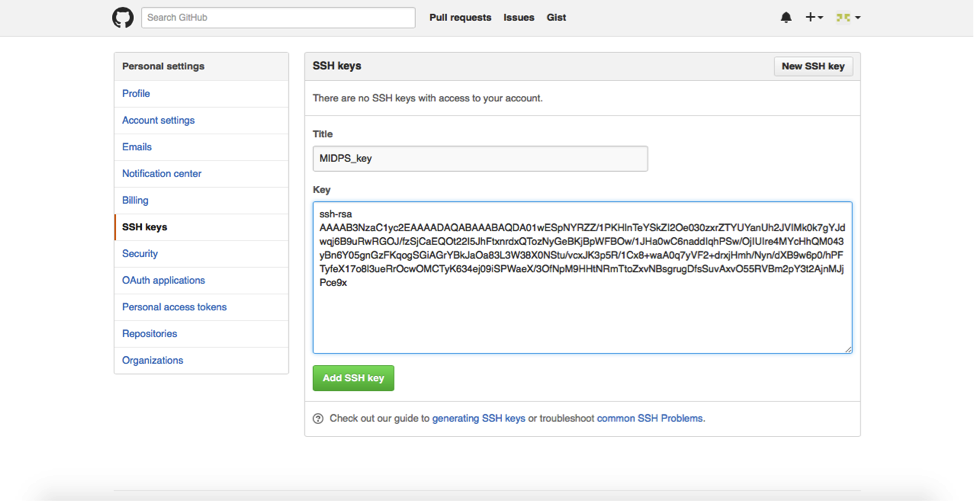
\includegraphics[width=15.5cm]{images/3}\\
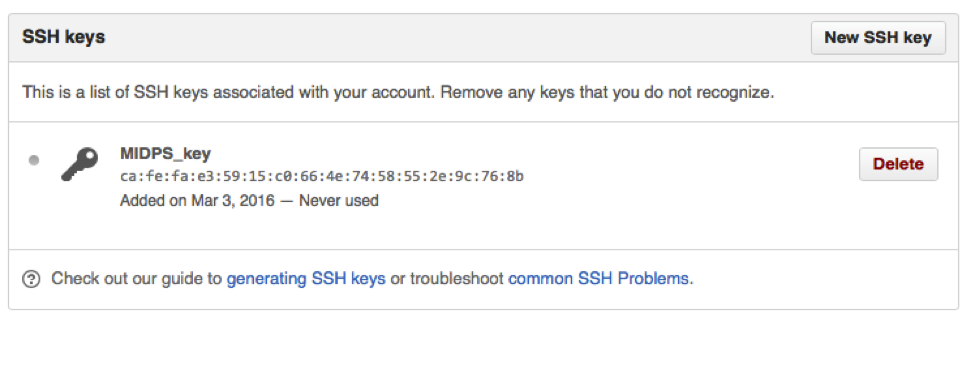
\includegraphics[width=15.5cm]{images/4}\\
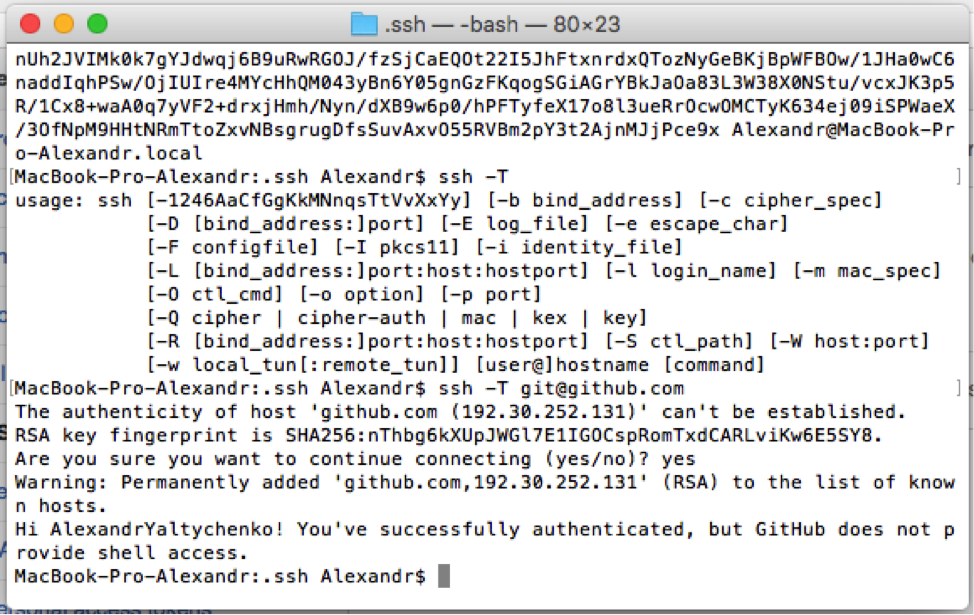
\includegraphics[width=12.5cm]{images/5}\\
\subsection{Clonarea repozitoriului gol creat pe github.com}
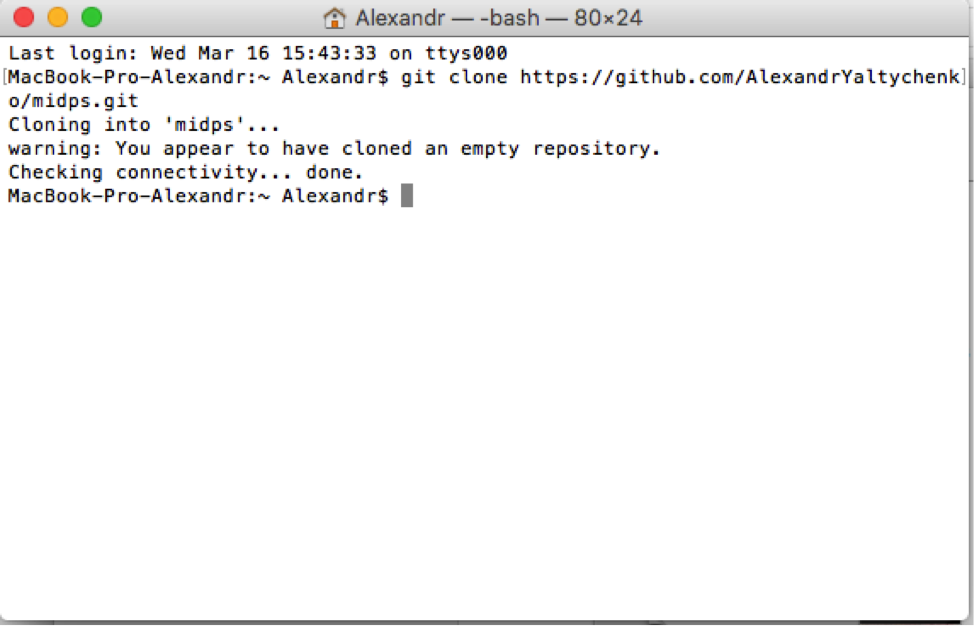
\includegraphics[width=12.5cm]{images/6}
\subsection{Crearea fișierului README in nano}
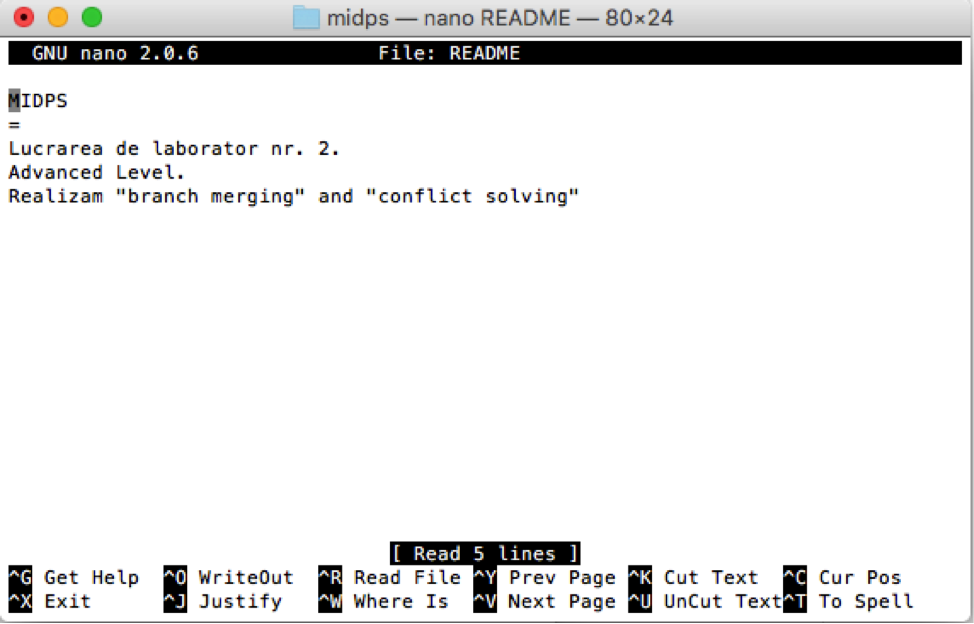
\includegraphics[width=12.5cm]{images/7}
\subsection{Crearea fisierului .gitignore in nano (ca sa fie  ignorat fisierul .DS\_Store generat de OS X)}
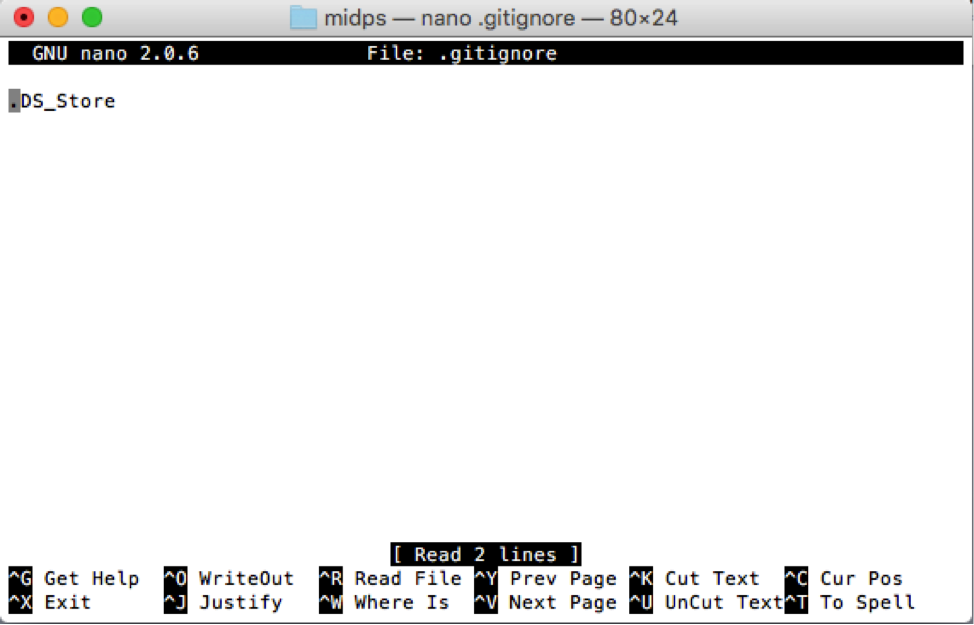
\includegraphics[width=12.5cm]{images/8}
\subsection{Desfășurarea primului add .}

\includegraphics[width=12.5cm]{images/9}
\subsection{Desfasurarea primului commit}
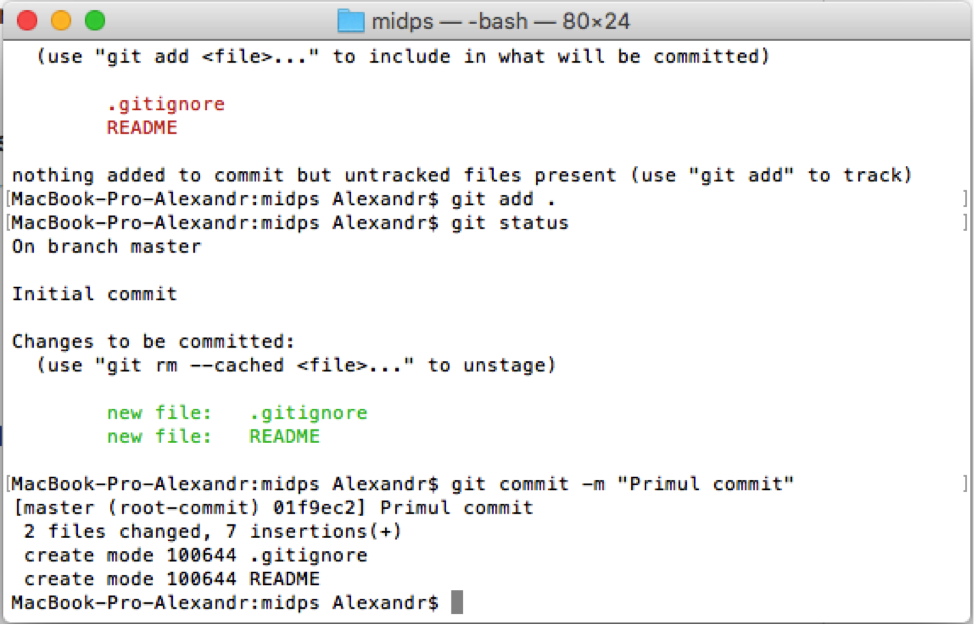
\includegraphics[width=12.5cm]{images/10}
\subsection{Desfasurarea primului push (Deci branch-ul to track a remote origin a fost setat cu succes)}
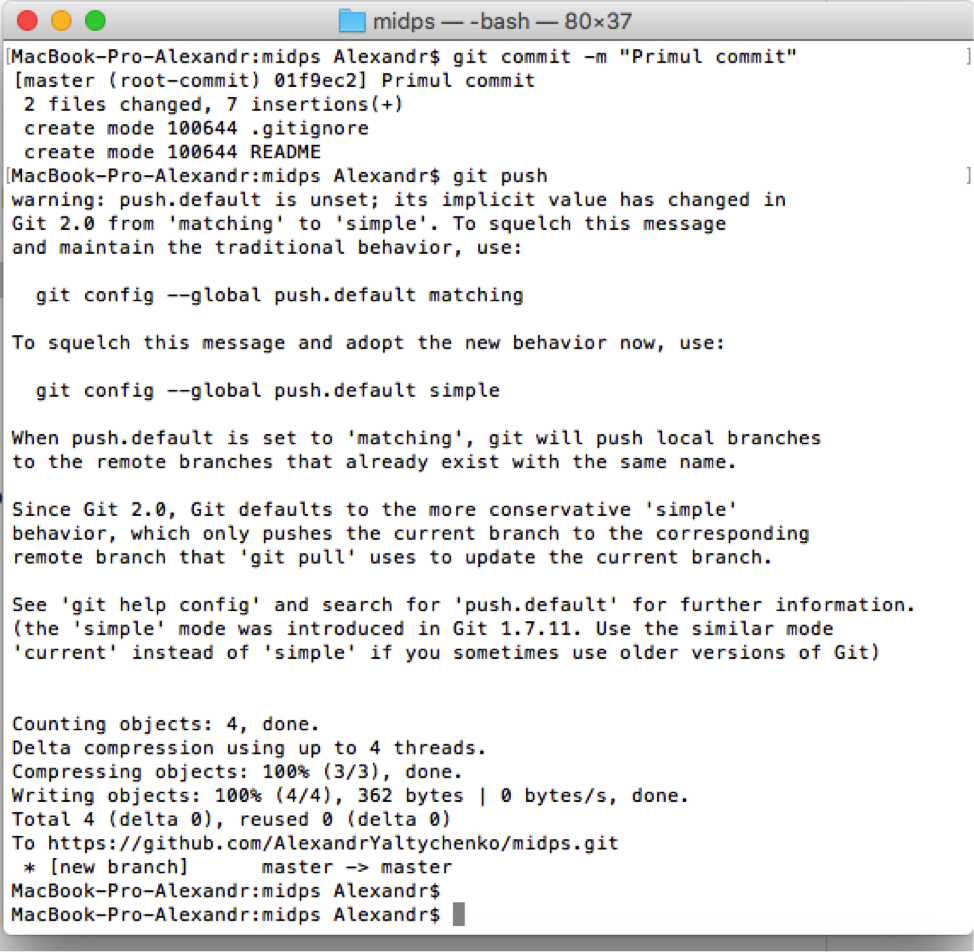
\includegraphics[width=12.5cm]{images/11}
\subsection{Adaugarea unui nou fisier hello.java la repozitoriul github}
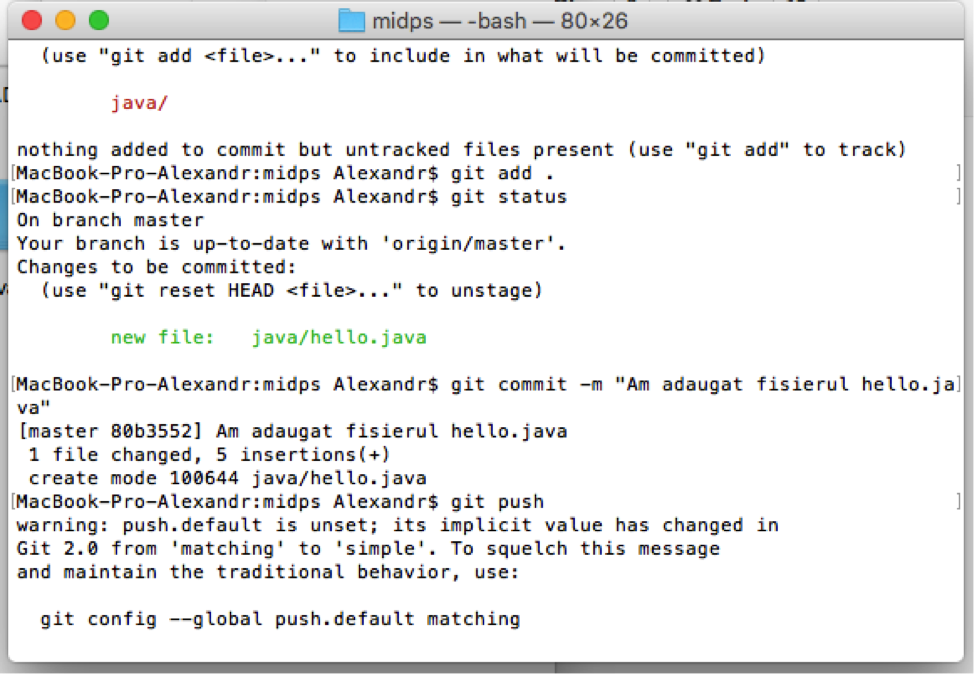
\includegraphics[width=12.5cm]{images/12}\\
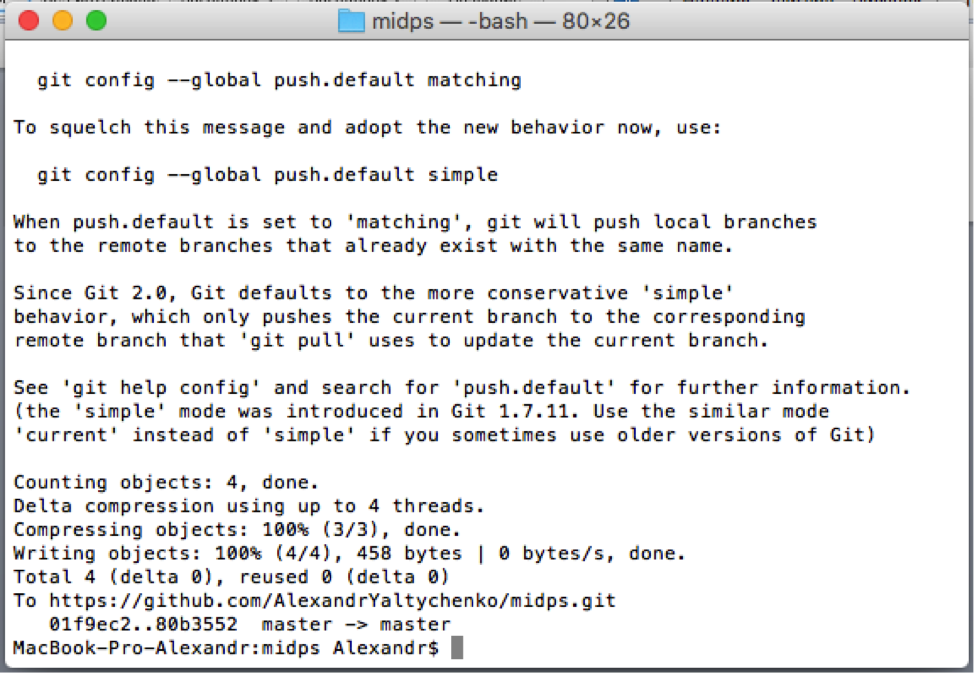
\includegraphics[width=12.5cm]{images/13}
\subsection{Editarea mesajului afisat in hello.java}
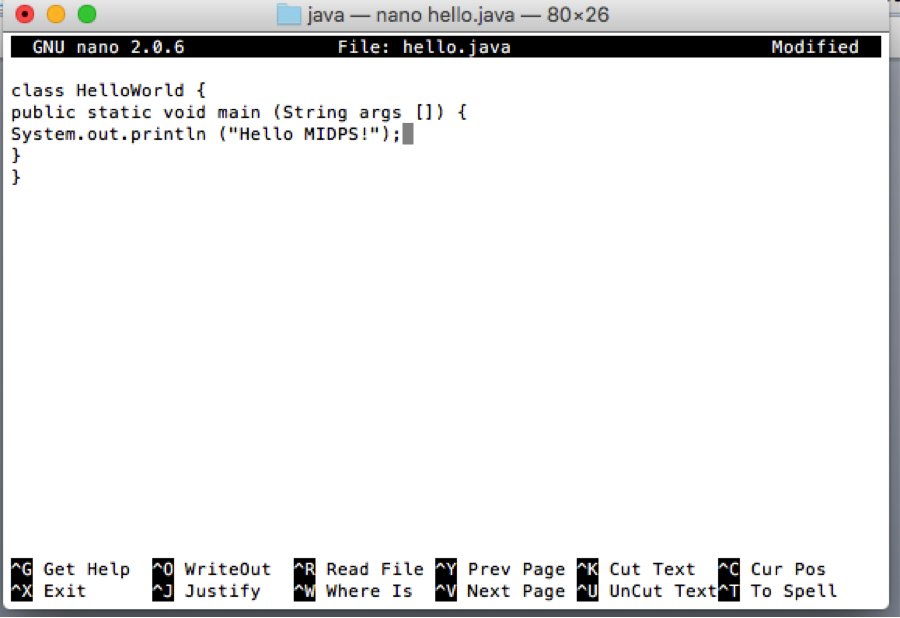
\includegraphics[width=12.5cm]{images/14}
\subsection{Inca un commit si push}
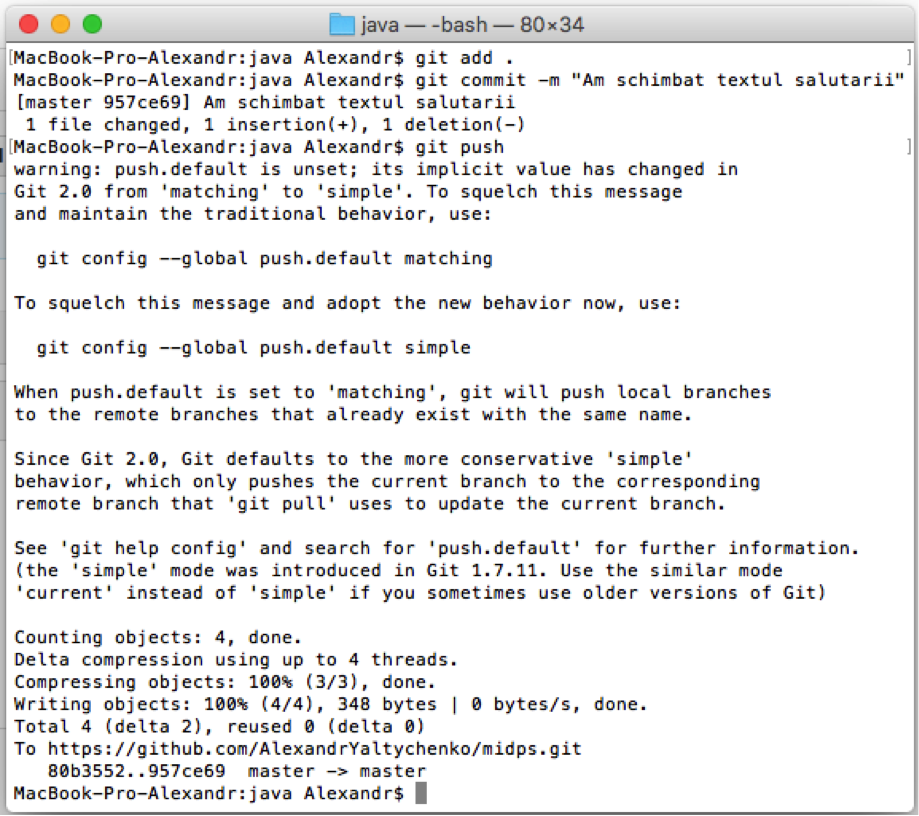
\includegraphics[width=12.5cm]{images/15}
\subsection{Implementarea recomandarilor lui git pentru ca warning-urile sa nu fie afisate}
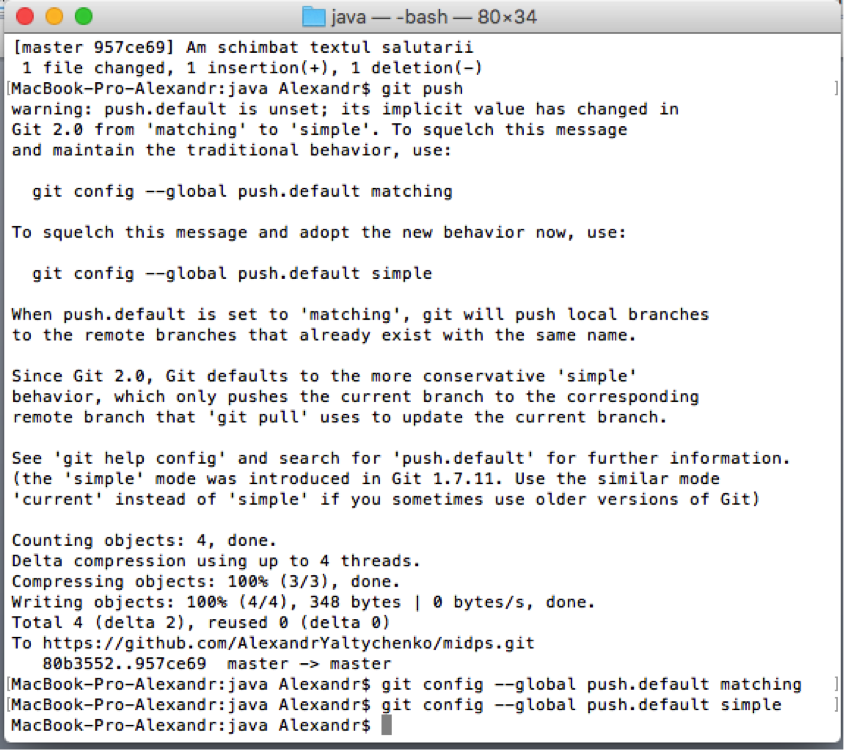
\includegraphics[width=12.5cm]{images/16}
\subsection{Crearea branch-ului ‘another’ și selectarea acestuia}
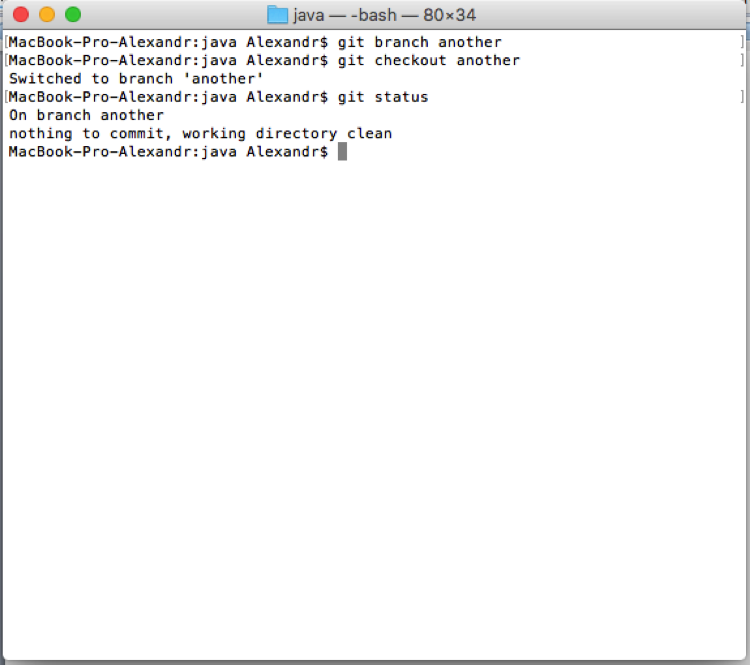
\includegraphics[width=12.5cm]{images/17}
\subsection{Gasirea solutiei pe Stack Overflow cum poate fi usor indeplinita resetarea ultimului commit}
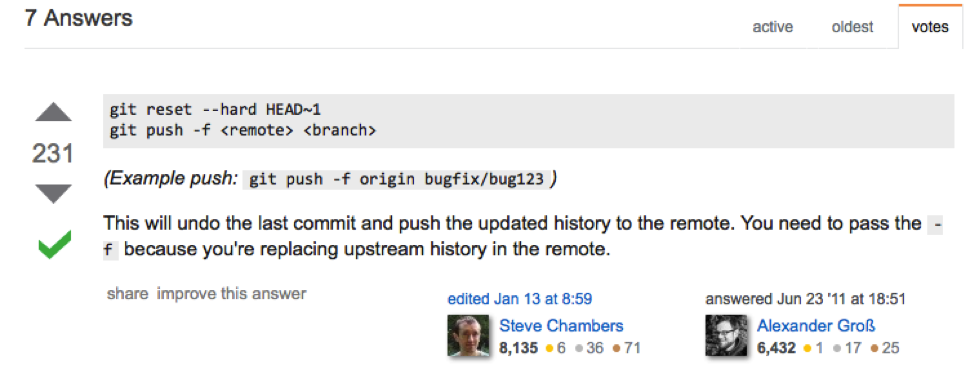
\includegraphics[width=12.5cm]{images/18}
\subsection{Verificarea git-log-ului al branch-ului ‘another’ si resetarea ultimului commit}
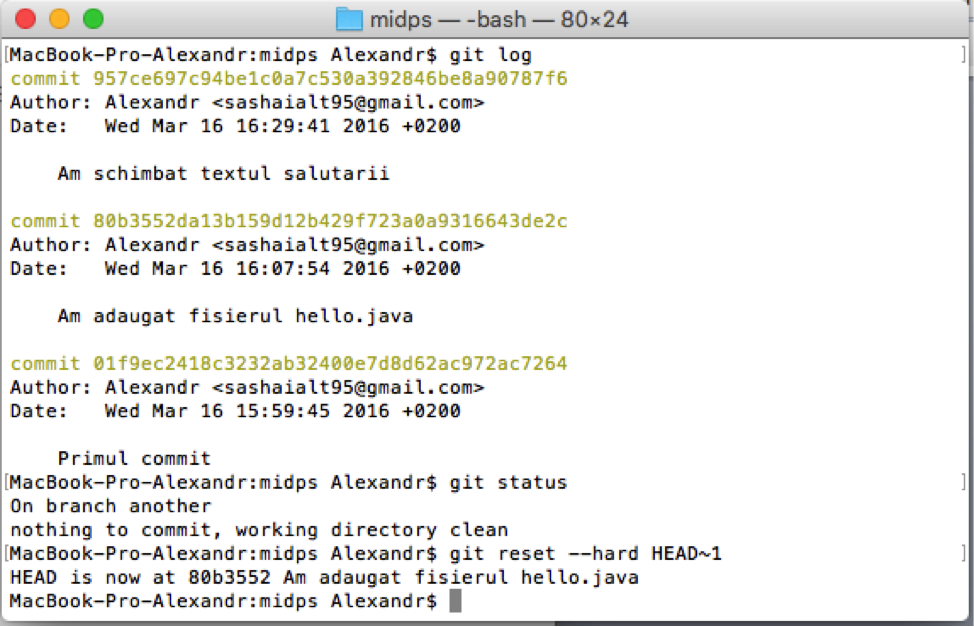
\includegraphics[width=12.5cm]{images/19}
\subsection{Inca un push}
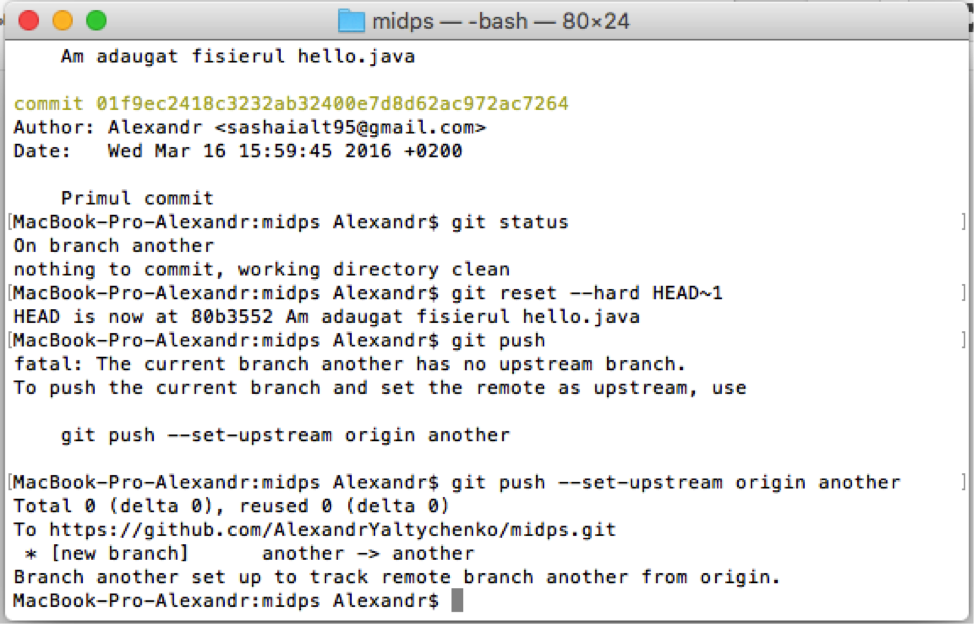
\includegraphics[width=12.5cm]{images/20}
\subsection{Inca o editare a fisierului hello.java (branch-ul ‘another’)}
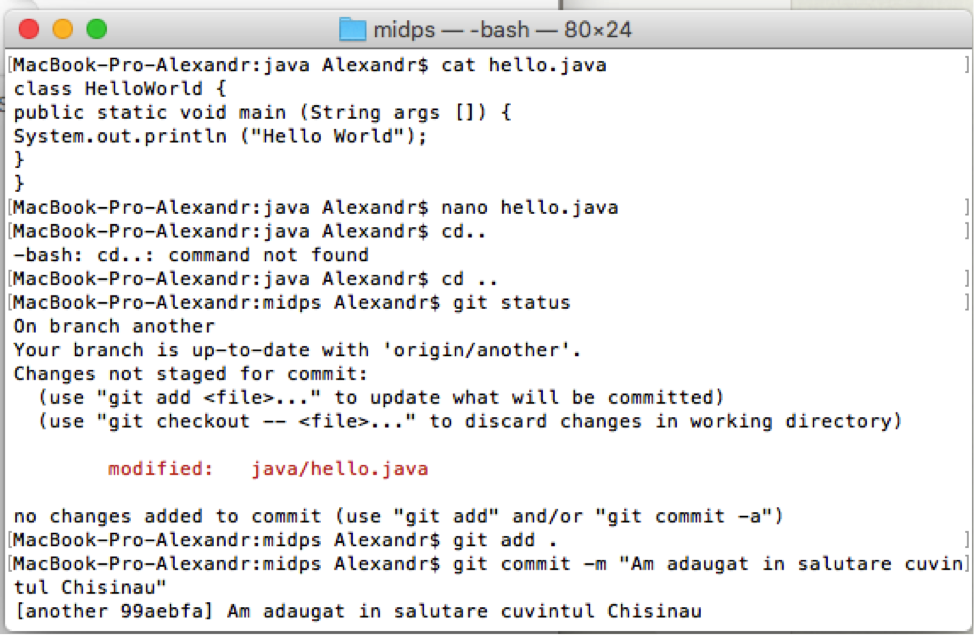
\includegraphics[width=12.5cm]{images/21}
\subsection{Selectarea branch-ului ‘master’}
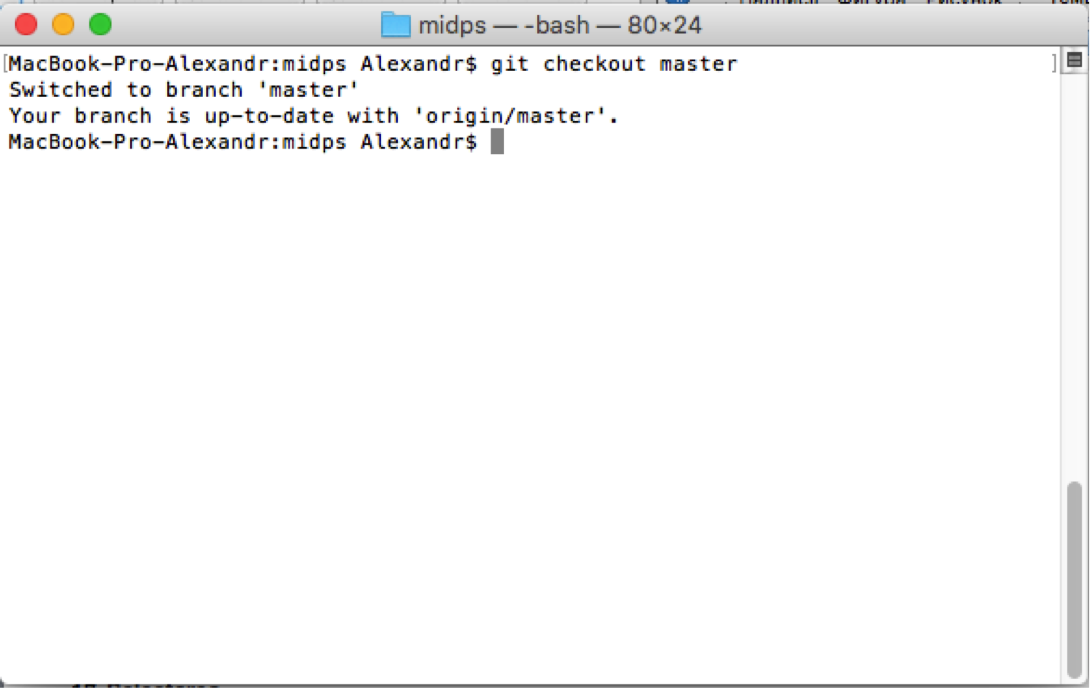
\includegraphics[width=12.5cm]{images/22}
\subsection{Verificarea log-ului si “branch merging” (apare conflictul)}
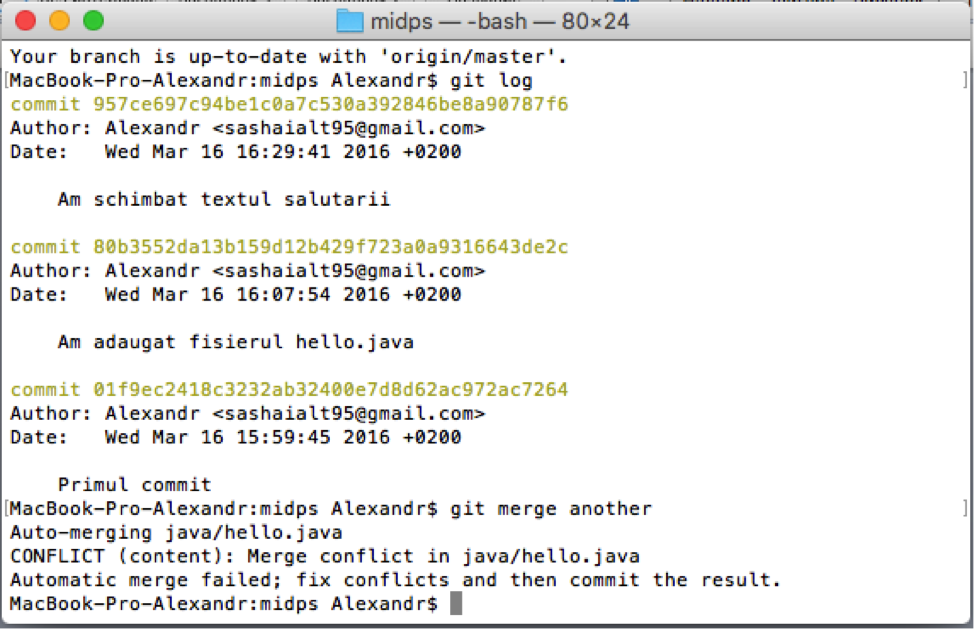
\includegraphics[width=12.5cm]{images/23}
\subsection{Solutionarea confilctului prin editarea fisierului hello.java}
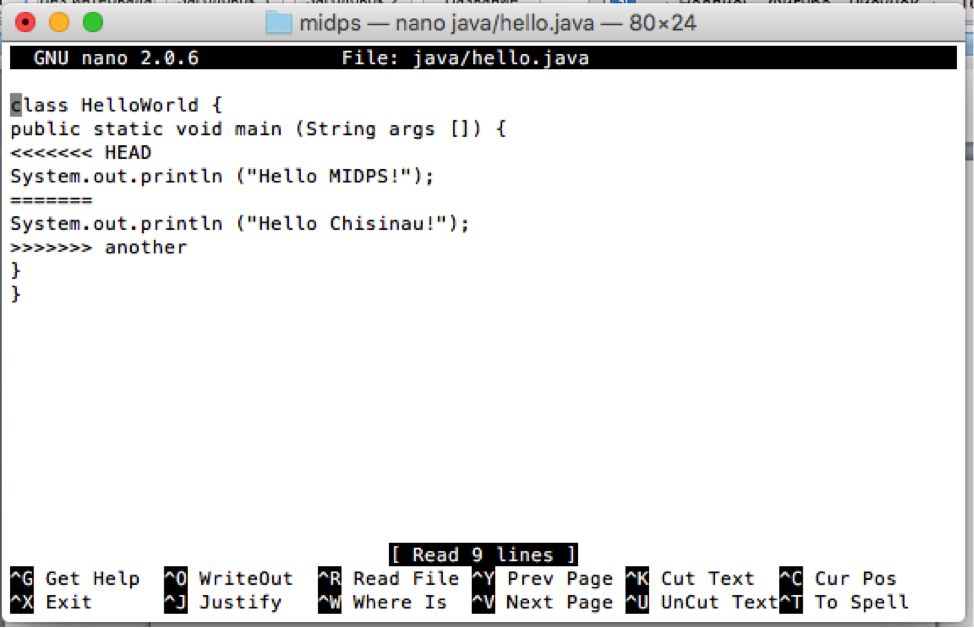
\includegraphics[width=12.5cm]{images/24}\\
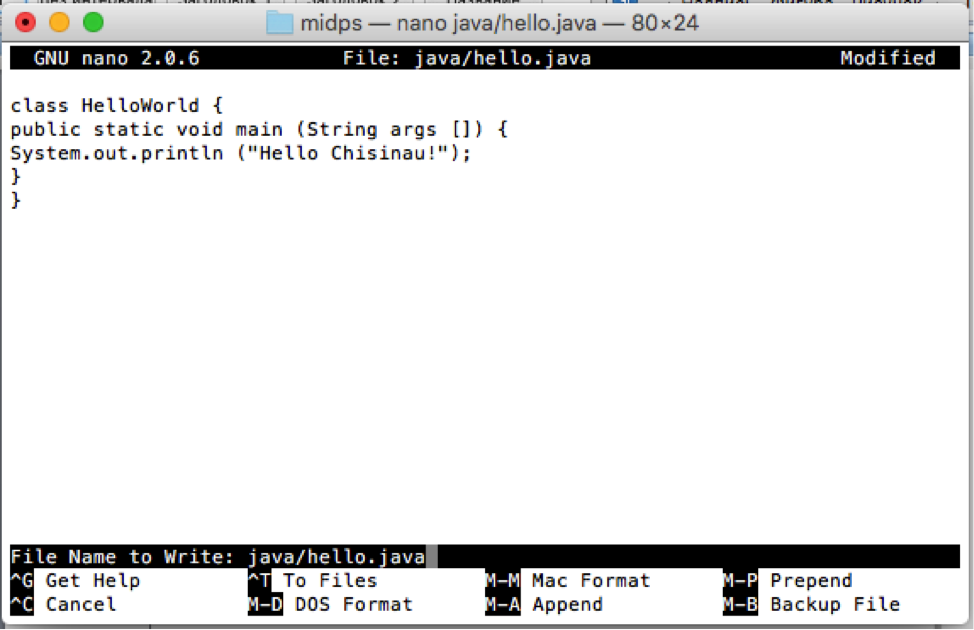
\includegraphics[width=12.5cm]{images/25}
\subsection{Terminarea procesului de «branch merging»}
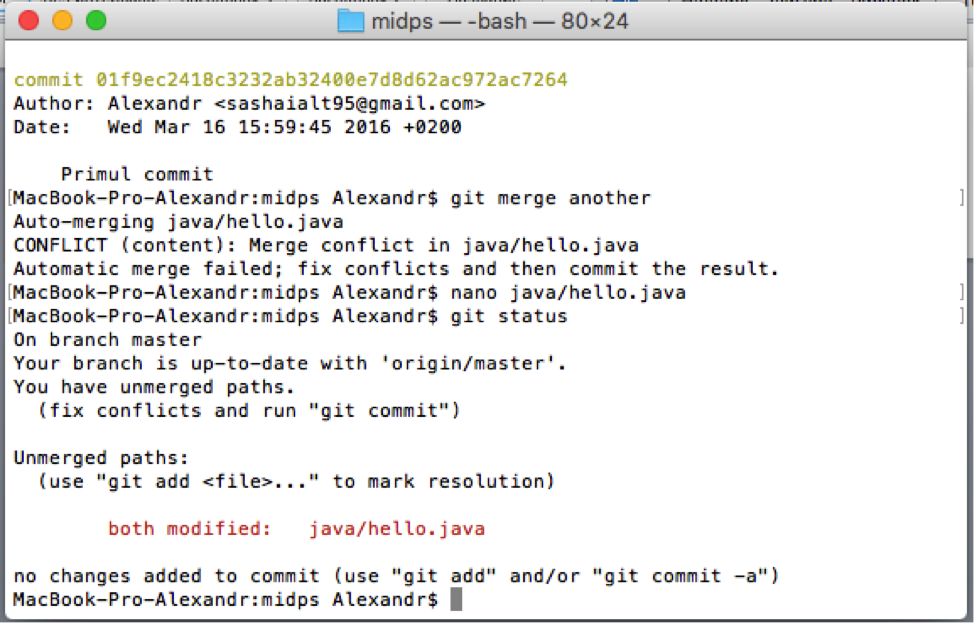
\includegraphics[width=12.5cm]{images/26}\\
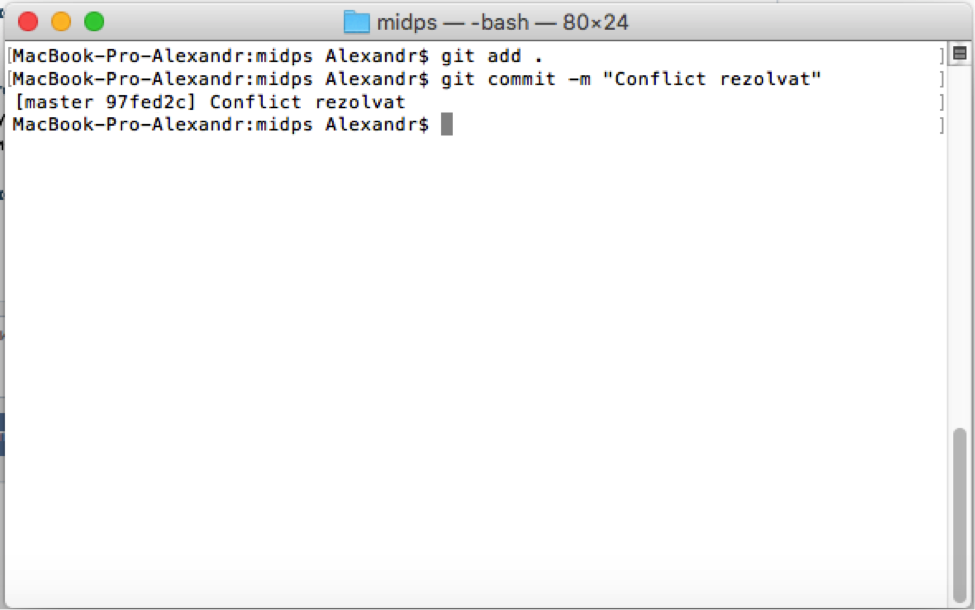
\includegraphics[width=12.5cm]{images/27}
\section {Bonus Point}
\textbf{Bash-script-ul pentru compilarea hello-world-urilor in limbaje C, Java, C++, Python:}\\

\begin{lstlisting}
#!/bin/bash
gcc hello_c.c -o hello_c
javac hello_java.java
g++ hello_c++.cpp -o hello_c++
python -m py_compile hello_python.py
\end{lstlisting}

\section*{Concluzii}
In cadrul acestei lucrari de laborator am studiat principiile si modul de utilizare a sistemului de control al versiunilor – Git. Prin intermediul CLI am configurat SSH autentificarea, am facut primul git commit și am sincronizat dispozitoriul local cu cel remote, plasat pe server. Mai departe am reusit sa fac “branch merging” si solutionez conflictul care a aparut. Cunoștintele, obtinute pe parcursul desfasurarii lucrarii de laborator vor fi foarte utile pentru realizarea proiectelor, ce urmeaza.
\section*{Bibliografie}
\begin{enumerate}
	\item https://training.github.com/kit/downloads/github-git-cheat-sheet.pdf - \textbf{Git Cheat Sheet}
\end{enumerate}





\end{document}